\section{Results}

The author permitted to see the grand academy of Lagado.  The academy largely described.  The arts wherein the professors employ themselves.

\begin{figure}
\begin{subfigure}{.5\linewidth}
\centering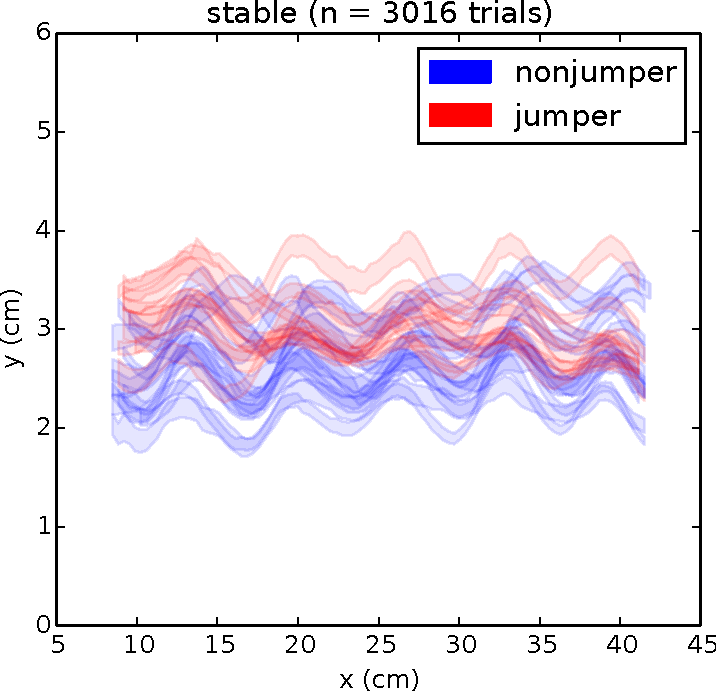
\includegraphics[width=\columnwidth]{chapters/figuresChBehaviour/noseTrajectoryStable}
\label{fig:noseTrajectoryStable}
\end{subfigure}%
\begin{subfigure}{.5\linewidth}
\centering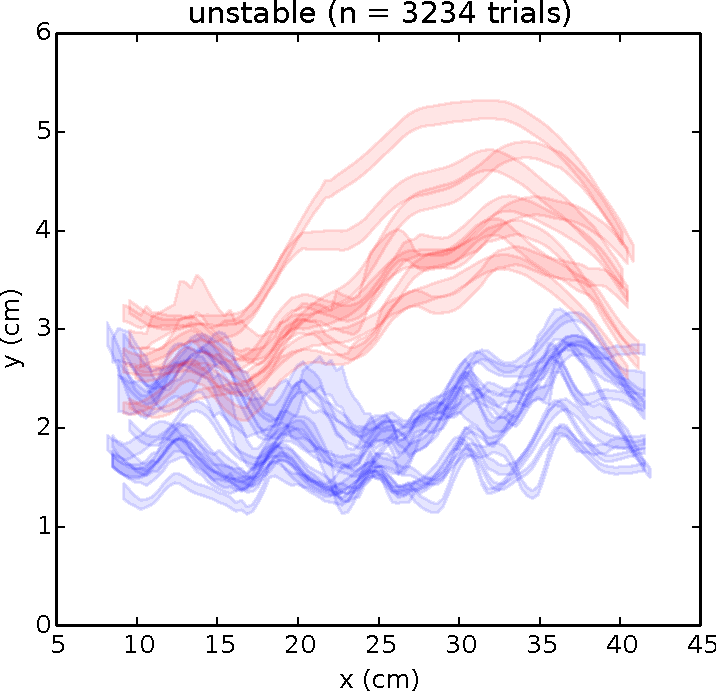
\includegraphics[width=\columnwidth]{chapters/figuresChBehaviour/noseTrajectoryUnstable}
\label{fig:noseTrajectoryUnstable}
\end{subfigure}\\[1ex]
\begin{subfigure}{\linewidth}
\centering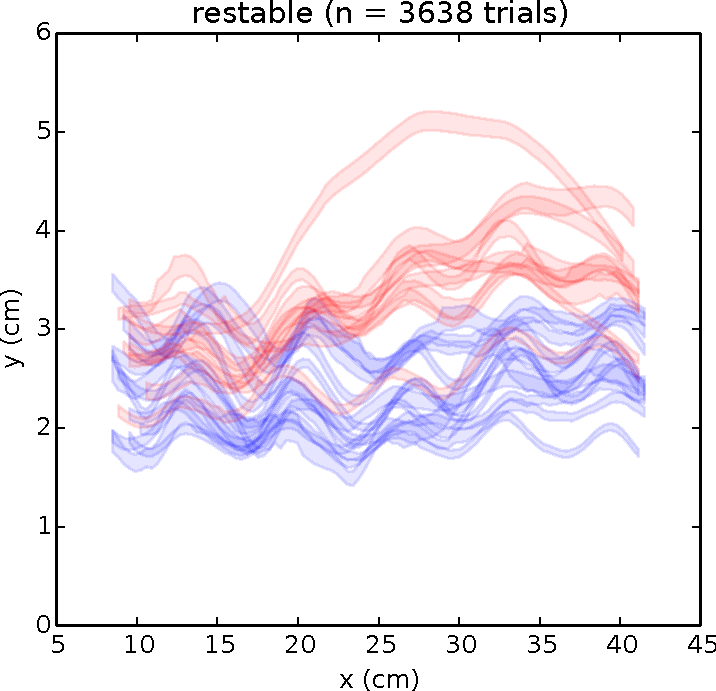
\includegraphics[width=.5\columnwidth]{chapters/figuresChBehaviour/noseTrajectoryRestable}
\label{fig:noseTrajectoryRestable}
\end{subfigure}
\caption{\textbf{Average nose trajectories when crossing the obstacles under different conditions of the shuttling protocol.} Each line represents the average nose trajectory for each individual animal. Line thickness indicates standard error of the mean. Leftward trials were mirrored so that progression is always from left to right. Classification of an animal into jumper or non-jumper was done on the basis of their trajectory in the \emph{unstable} condition and retained throughout.}
\label{fig:noseTrajectory}
\end{figure}

% \begin{figure}
% \begin{center}
% \includegraphics[width=\columnwidth]{chapters/figuresChBehaviour/nosetrajectory}
% \end{center}
% \vspace{-5mm}
% \caption{\textbf{Average nose trajectories when crossing the obstacles under different conditions of the shuttling protocol.} Each line represents the average nose trajectory for each individual animal. Line thickness indicates standard error of the mean. Leftward trials were mirrored so that progression is always from left to right. Classification of an animal into jumper or non-jumper was done on the basis of their trajectory in the \emph{unstable} condition and retained throughout.}
% \label{fig:nosetrajectory}
% \end{figure}